\documentclass[12pt]{article}\usepackage[]{graphicx}\usepackage[]{color}
% maxwidth is the original width if it is less than linewidth
% otherwise use linewidth (to make sure the graphics do not exceed the margin)
\makeatletter
\def\maxwidth{ %
  \ifdim\Gin@nat@width>\linewidth
    \linewidth
  \else
    \Gin@nat@width
  \fi
}
\makeatother

\definecolor{fgcolor}{rgb}{0.345, 0.345, 0.345}
\newcommand{\hlnum}[1]{\textcolor[rgb]{0.686,0.059,0.569}{#1}}%
\newcommand{\hlstr}[1]{\textcolor[rgb]{0.192,0.494,0.8}{#1}}%
\newcommand{\hlcom}[1]{\textcolor[rgb]{0.678,0.584,0.686}{\textit{#1}}}%
\newcommand{\hlopt}[1]{\textcolor[rgb]{0,0,0}{#1}}%
\newcommand{\hlstd}[1]{\textcolor[rgb]{0.345,0.345,0.345}{#1}}%
\newcommand{\hlkwa}[1]{\textcolor[rgb]{0.161,0.373,0.58}{\textbf{#1}}}%
\newcommand{\hlkwb}[1]{\textcolor[rgb]{0.69,0.353,0.396}{#1}}%
\newcommand{\hlkwc}[1]{\textcolor[rgb]{0.333,0.667,0.333}{#1}}%
\newcommand{\hlkwd}[1]{\textcolor[rgb]{0.737,0.353,0.396}{\textbf{#1}}}%
\let\hlipl\hlkwb

\usepackage{framed}
\makeatletter
\newenvironment{kframe}{%
 \def\at@end@of@kframe{}%
 \ifinner\ifhmode%
  \def\at@end@of@kframe{\end{minipage}}%
  \begin{minipage}{\columnwidth}%
 \fi\fi%
 \def\FrameCommand##1{\hskip\@totalleftmargin \hskip-\fboxsep
 \colorbox{shadecolor}{##1}\hskip-\fboxsep
     % There is no \\@totalrightmargin, so:
     \hskip-\linewidth \hskip-\@totalleftmargin \hskip\columnwidth}%
 \MakeFramed {\advance\hsize-\width
   \@totalleftmargin\z@ \linewidth\hsize
   \@setminipage}}%
 {\par\unskip\endMakeFramed%
 \at@end@of@kframe}
\makeatother

\definecolor{shadecolor}{rgb}{.97, .97, .97}
\definecolor{messagecolor}{rgb}{0, 0, 0}
\definecolor{warningcolor}{rgb}{1, 0, 1}
\definecolor{errorcolor}{rgb}{1, 0, 0}
\newenvironment{knitrout}{}{} % an empty environment to be redefined in TeX

\usepackage{alltt}
%Required: You must have these
\usepackage{graphicx}
\usepackage{tabularx}
\usepackage{natbib}

\usepackage{array}
\usepackage{amsmath}
%\usepackage[backend=bibtex]{biblatex}
\setkeys{Gin}{width=0.8\textwidth}
%\setlength{\captionmargin}{30pt}
\setlength{\abovecaptionskip}{10pt}
\setlength{\belowcaptionskip}{10pt}
 \topmargin -1.5cm 
 \oddsidemargin -0.04cm 
 \evensidemargin -0.04cm 
 \textwidth 16.59cm
 \textheight 21.94cm 
 \parskip 7.2pt 
\renewcommand{\baselinestretch}{1.2} 	
\parindent 0pt

\bibliographystyle{..//..//refs/bibstyles/amnat.bst}
\usepackage{xr-hyper}
\usepackage{hyperref}


\title{Continental divides: Spring climate variability shapes the phenological cue strength of woody species in temperate North America, not Europe\\ or\\
Spring climate stability shapes phenological cue sensitivities of temperate forest in North America but not Europe\\ or\\
Limited support for range-wide climate patterns shaping phenological cue differences among woody plants of temperate North America and Europe \\or\\
Other
}

\author{Dan, Cat, Nacho and Lizzie and the lab}
\IfFileExists{upquote.sty}{\usepackage{upquote}}{}
\begin{document}
\maketitle

\section*{Abstract}
\section*{Introduction}
\textbf{For woody plants of the temperate zone the phenology, or annual timing, of spring budburst influences a myriad of ecological processes including patterns of resource allocation \citep{}, trophic interactions \citep{} and biogeochemical cycling \citep{}.}
 Through budburst timing, woody plants balance the advantages of precocious growth resumption for resource gains with the risk of damage from late season frost \citep{}. To navigate this tradeoff, woody plants have evolved complicated networks of sensory organs, hormone signaling, and physiological responses to sense environmental cues; changes in their physical environment, that signal the arrival of appropriate conditions for resuming growth.\\

\textbf{Decades of research suggest that warming spring temperatures (forcing), cool winter temperatures (chilling) and day length (photoperiod) are primary environmental cues utilized by woody plants that determine the timing of spring phenological events \cite{}}. These studies also demonstrate the there are substantial cue-use differences among species, with some species relying more heavily on some cues over others \citep{Laube:2014aa}. As anthropogenic climate change has already driven shifts in spring phenology \citep{}, identifying these inter-specific differences in cue use has emerged as a major goal of phenological research \citep{}. These differences have strong implications for both predicting the rate of phenological shifts as the climate continues to warm \citep{}, and anticipating the ecological consequences of these shifts \citep{}.

\textbf{ But the quantification of cue use difference among species offers even more---a novel opportunity to interrogate long-standing theories regarding the biology underlying cue-use difference among species.} One particular relationship that can now be examined this the relationship species' geographic ranges and phenological cue use.

Climate is the major selective force on both species' geographic ranges \citep{} and their phenology \citep{}, and therefore, it is widely assumed that phenological cue-use differences among species reflect the climate of their respective ranges \citep{}. That is, a species' relative reliance on forcing, chilling and photoperiod for should be shaped by the unique environmental conditions across a species' geographic range.\\

Despite this intuitive link between climate and cues, direct tests of this assumption are rare ( but see \citep{Zohner:2017aa}). With the recent quantification for cue use of many species \citep{} and the accessibility of high resolution climate data it is now possible to rigorously test this theory with data. Below, we briefly outline two hypotheses presented in the literature about the relationship between phenological cue-use and species' climatic range characteristics. We then test these predictions using Bayesian models for a large suite of temperate woody species from North America and Europe.


\subsection{Climate intensity hypothesis}
One hypothesis for the evolution of cue use differences across species is that species utilize the climate cues to which they have the most exposure. Simply stated, there should be a positive correlation between the amount or intensity of a cue across a species' range and the species phenological sensitivity to that cue. This hypothesis predicts that species with  a) high numbers growing degree days in their range should have stronger forcing cues, b) higher amount of chilling should have stronger chilling cues and c) more annual photoperiod variation should have stronger photoperiod cues. This hypothesis has been applied to explain large, macro-ecological patterns in phenology like why the tropical phenology cues primary to forcing and temperate and arctic phenology is more dependent on photoperiod and/or chilling \citep{} but has not been widely tested within biomes for species with overlapping ranges.  

\subsection{Climate variability hypothesis}

Current understanding of the evolution of phenological cues assume that forcing is the predominant cue. In this framework,a secondary reliance on photoperiod and/or chill cues evolve when forcing alone is not a reliable cue of safe growing condition \citep{Korner:2010aa}. Forcing is is an unreliable cue when temperatures unstable in the spring time. The climate variability hypothesis predicts species with high variation in spring temperature in there range should evolve a stronger response to all three cues, especially chilling and or photoperiod,  \citep{Wang:2014aa, Muffler2016}. This hypothesis potentially explains the stronger cue sensitivity of temperate North American species to those in Europe where there is less climate variability in the spring \citep{Zohner}.

However, a major hurdle to robustly testing this hypothesis is that, when considered in the context of a species' geographic range, spring temperature variation occurs on multiple temporal and spatial scale. Phenology may be shaped by intra-annual temperature variation (e.g. frequency of late season frost, diurnal temperature functions), inter-annual variation (e.g. annual mean temperatures) and the interaction between them (e.g. inter-annual variation in last season frost episodes). Further, each of the level of variation be quite different across a species range, suggesting geographic variation with the range must also be accounted for.
Any of these level of variation could itself drive selection for secondary cue usage (photoperiod/chilling), and it is unclear how they interact or which is most important \citep{Zagmajster:2014aa}. Key to testing the climate variability hypotheses is to first characterize relationships between spring temperature variation at multiple spatio-temporal scales.

\subsection{Local climate hypothesis}
An implicit assumption of the previously stated hypotheses is that among species cue-use variation is higher than within species (ie cue use is ``conserved" at the species level). If rather, cue use patterns are locally adapted, while climate intensity and climate variability may still drive cue-use patterns at the population level, it would be difficult to detect consistent patterns across a species full geographic range. There is not yet a strong consensus about to what degree cue use is locally adapted and it likely varies between phenophases \citep{}, and organisms \citep{}. As such, any analysis considering species ranges and cue use must account for intra-specific differences as well.

\subsection{Non-climate drivers of cue use}
It is also important to recognize that though climate is the mechanism underlying woody plant phenology, there may be other selective forces driving cue use. Cue use differences may be the product of other tradeoffs. Could say this here or leave for the discussion.

We leveraged over 50 years worth of phenology experiments in the OSPREE database \citep{} and climate data collected across the ranges of temperate woody species in North America and Europe to test the three major climate-cue use hypotheses. We used a Bayesian hierarchical approach to jointly fit models estimating of forcing, chilling and photoperiod sensitivity for each species and the effects of several dimensions of climate intensity and variability in the species ranges on these estimates. Then for a subset of well represented species in our dataset, we modeled the among and within species variation in cue use to quantify the relative strength of local adaptation of pattern of phenological cue use. With this approach we 1) clarify the relationships between climatic variability across multiple scales of spatio-temporality, 2) identify the climate drivers that are more and less likely to drive selection on phenological cues and 3) compare variation in cue-use among and within species and between temperate Europe and North America. Our interrogation of these relationships between climate and cue use not only elucidates the evolutionary drivers of phenoloical cues, but offers new insights regarding implications of climate change as both species' ranges and phenology continue to shift with warming.

\section*{Methods}
\subsection*{Phenological data and cue-use estimates}
Dan and/or Lizzie write:
\begin{itemize}
\item Introduce OSPREE
\item Species selection
\item Model description
\end{itemize}

\subsection*{Species' range characteristics}
Cat and/or Nacho write?\\
\begin{itemize}
\item Climate data \textbf{(Figure of range maps with one climate variable, other could go to supplement)}
\item note on temp vs. geographic variation
\item calculation of GDD last frost
\item STV

\end{itemize}

\subsection*{Statistical analysis}
\subsubsection*{Coherance of climate variability}
\subsubsection*{climate cue-use relationships}
Dan write description of joint model

\subsubsection*{Intra vs. interspecific models}
Cat 






\section*{Results}
\subsection*{Climate intensity and cue use}
Overall, the mean forcing (GDDs) and chilling (Chill Portions) had weak effects on estimated cue use. 
In our full species models mean GDDs and had a weakly negative or neutral association with cue strength (GDD:Chill=X ,GDD:Force=Y, GDD:Photo=Z, (Fig. \ref{fig:mods1 a),b)})). The general sign of these relationships persisted in the continent subset models (Fig. \ref{fig: mods1} d),e),f)) with the exception of the relationship between mean GDDs and chilling for North American species which became positive (mean= Z, (Fig. \ref{fig: mods1} c)). Generally, there was high uncertainty around these estimates suggesting climate intensity is a poor predictor for cue use. 

\subsection*{Coherance of spatio-temporal spring climate variability}
The spatio-temporal coherence of spring climate variability and intensity varied across continent and scales. Generally climate intensity (mean GDDs in range mean Chill Portions in range and Mean GDDs to last frost) were well correlated with climate variability (Fig. \ref{fig:corrs}a),b),c),d),h)) though strong differences can be observed between North American and Europe.  Intra-annual, inter-annual and spatial variability in spring climate were also well correlated  (Fig. \ref{fig:corrs}e),f),g)), though the variability of spring climate in Europe was very low, suggesting that these correlation are likely more relevant in North America.

\subsection*{Climate variation and cue use}
In our full models, variation in growing degree days before the last frost of the season was weakly positively associated with forcing and photoperiod sensitivity and negatively associated with chilling sensitivity (Fig. \ref{fig:mods2}a))). However, our continent subset models shows different effect. The effect of Variation in GDDs to last frost is poorly estimated in the European data subset,and has almost no effect on cue use over the narrow range of spring cliamte varaition present in Europe  (Fig. \ref{fig:mods2}b). In the North America subset, variation in GDD to last frost increases sensitivity in all three cues (Chilling:X Forcing:Y Photoperiod:Z, (Fig. \ref{fig:mods2}c))) suggesting there may be support for the climate variation hypotheses in North America where spring climate variation can be extreme. We found qualitatively similar continental patterns in the relationships between cue-use and climate variability  using STV as an alternative metric inter-annual variation (SUPP).

\subsection*{Local adaptation of phenological cues}
We detected limited population level variation in forcing and photoperiod cue sensitivity, though this within species variation was less substantial than among species variation(Fig. \ref{fig:popy}). Notably, we found the largest source of variation in phenological was

\subsection{Cue use in North America and Europe}
We found that the strength of secondary cue use (chilling and photoperiod) was higher in North America than in Europe (Chilling: NA-X, EU-Y, Photoperiod NA-X, EU-Y,Fig.\ref{fig:contcues}), while forcing sensitivity was higher in Europe than North America (NA-X, EU-Y). This result is consistent with the observation that the spring climate of North America is much less stable than Europe and our finding that the climate-cue use hypotheses appear to be better supported in North America.

\section*{Discussion}
Mian points:
\begin{enumerate}
\item cliamte patterns: scales of variation and Climate differences
\item Our finding are in line with Zohner but more stark... Relevance in N.A. but NOT Europe
\item Implications: Cross continental comparisons of limited utility. Consider other hypotheses
\item More data!
\end{enumerate}

Our investigation of the relationship between the climate in range of species and their phenological cue use revealed several insight about large scale patterns about climatic and biological patterns across the temperate zone, and the relationship between them. Considering climate alone, we found strong coherence between temporal and spatial climate variability across a species range. This high autocorrelation in spatio-temporal variability is useful for future studies but we can probably say something better here. Any ideas? \\

Our study also highlights that patterns of temperature variation and intensity are much stronger in temperate North America in Europe. This is a well meteorological phenomenon drive by large local climate pattern like the jet steam and enso and stuff (say better), but when combined with our biological findings, about cue use differences among taxa in North America vs. Europe, it is clear that this stark contrast must be better accounted for in understanding the evolutionary histories and ecological trajectories of the flora of these two continents.\\

Similar to previous studies, we found  stronger support for the climate variability hypothesis than the climate intensity hypothesis and that this influence of climate variability on cues use was high in North America \citep{}. While mean growing degree days in the range were positively associated with forcing sensitivity in North America as predicted by the climate intensity hypotheses, mean GDDs were also strongly associated with chilling sensitivity (Fig \ref{fig:mod1},d) but chilling sensitivity has no clear relationship with mean chilling in the range (Fig \ref{fig:mod1},f). Further there is high uncertainty surrounding the estimates in our climate intensities models suggest climate intensitiy is a poor predictor of phenological cue use. By contrast, climate variability increased the forcing, chilling and photoperiod sensitivities in North America (Fig \ref{fig:mod1},c) as predicted by the climate variability hypothesis, while there was virtually no relationship between climate variablility and cue use in European species.

While previous work has suggested that climate variability drive cue use differences between North America and Europe, the absence of a relationship between climate variability and cue use we found in our European data subset suggests a slightly different formulation. Our work suggest that climate variability may drive cue use only in North America where variation is sufficiently high to drive selection and not in Europe where variation is more limited.  

The implications of this finding are several fold. While phenological data collected across Europe and North America are often utilized in tandem to test basic evolutionary and ecological theories, our finding supports the assertion of a growing number of researchers that given the differences in land use and geological history and contemporary and predicted climate change, that treating the flora of these two regions as discrete units may facilitate more nuanced understanding and precise predictions for temperate forest ecology ( I actually don't know if this is true).

The second implication of our findings is the field of phenology must continue to expand the range of hypotheses we test and consider regarding the evolution of phenological cues. Phenology should continue to draw from studies of paleoclimate, biogeography, evolutionary ecology and community ecology. There is a rich literature predicting that phenological cue differences among species may be the product of historic climate legacies \citep{}, strong phylogentic constraints or driven by community processes of phenological assembly like competition, niche theory  \citep{}. It is likely all of these factors along with the bioclimatic drivers we tested above drive selection on phenology and the the selection strength differs across time and space. Therefore, as we continue to gather more data on phenological cue use patterns for a more species, these hypotheses must be rigorously tested alongside the bioclimatic ones we address here.

Increasing the geographic and taxonomic breadth of phenological cue experiments is critical to understanding the evolution of phenological cues, and predicting how these interspecific differences in cues will impact forest ecology with global change. Despite utilizing one of the largest and species rich databases currently in existence for this study, there is still alot of noise (say better). In Both North America and Europe, the ranges of the species in our study we highly overlapping (make a mappy figure). It is possible that the influence of climate in range of species on differences in phenological cue use would be more pronounced for species with more discrete ranges (ie west vs. east coast of North America), but there is not currently enough taxonomic breadth in phenology to assess this.

Additionally, while we found that species level variation in cue use was higher than population level variation in our data, this finding was based on a limited subset of data because studies across many populations are rare. There is a live debate surrounding the degree to which woody plant phenology is driven by local adaptation \citep{}, and more data (say better) will be critical to address this.

In this study we found limited support for the assertion that the climate variables species experiences acorss their geographic ranges shape the relative reliance of forcing, chilling and photoperiod cues for spring phenology. Our results suggest that climate variability may drive cue use pattern only when it is sufficiently high, like in contemporary North America. These results suggests that future studies of phenolocial cue use would a holistic integration of these bioclimatic hypotheses with phylogenetic, functional trait, and climatic legacy hypotheses to fully understand the evolution of phenological cues in woody plants, and how cue use patterns will impact species performance in the face of global change at across multiple spatial and temporal scales.








\bibliography{..//..//refs/ranges}

\section*{Figures}

\begin{figure}[h!]
    \centering
 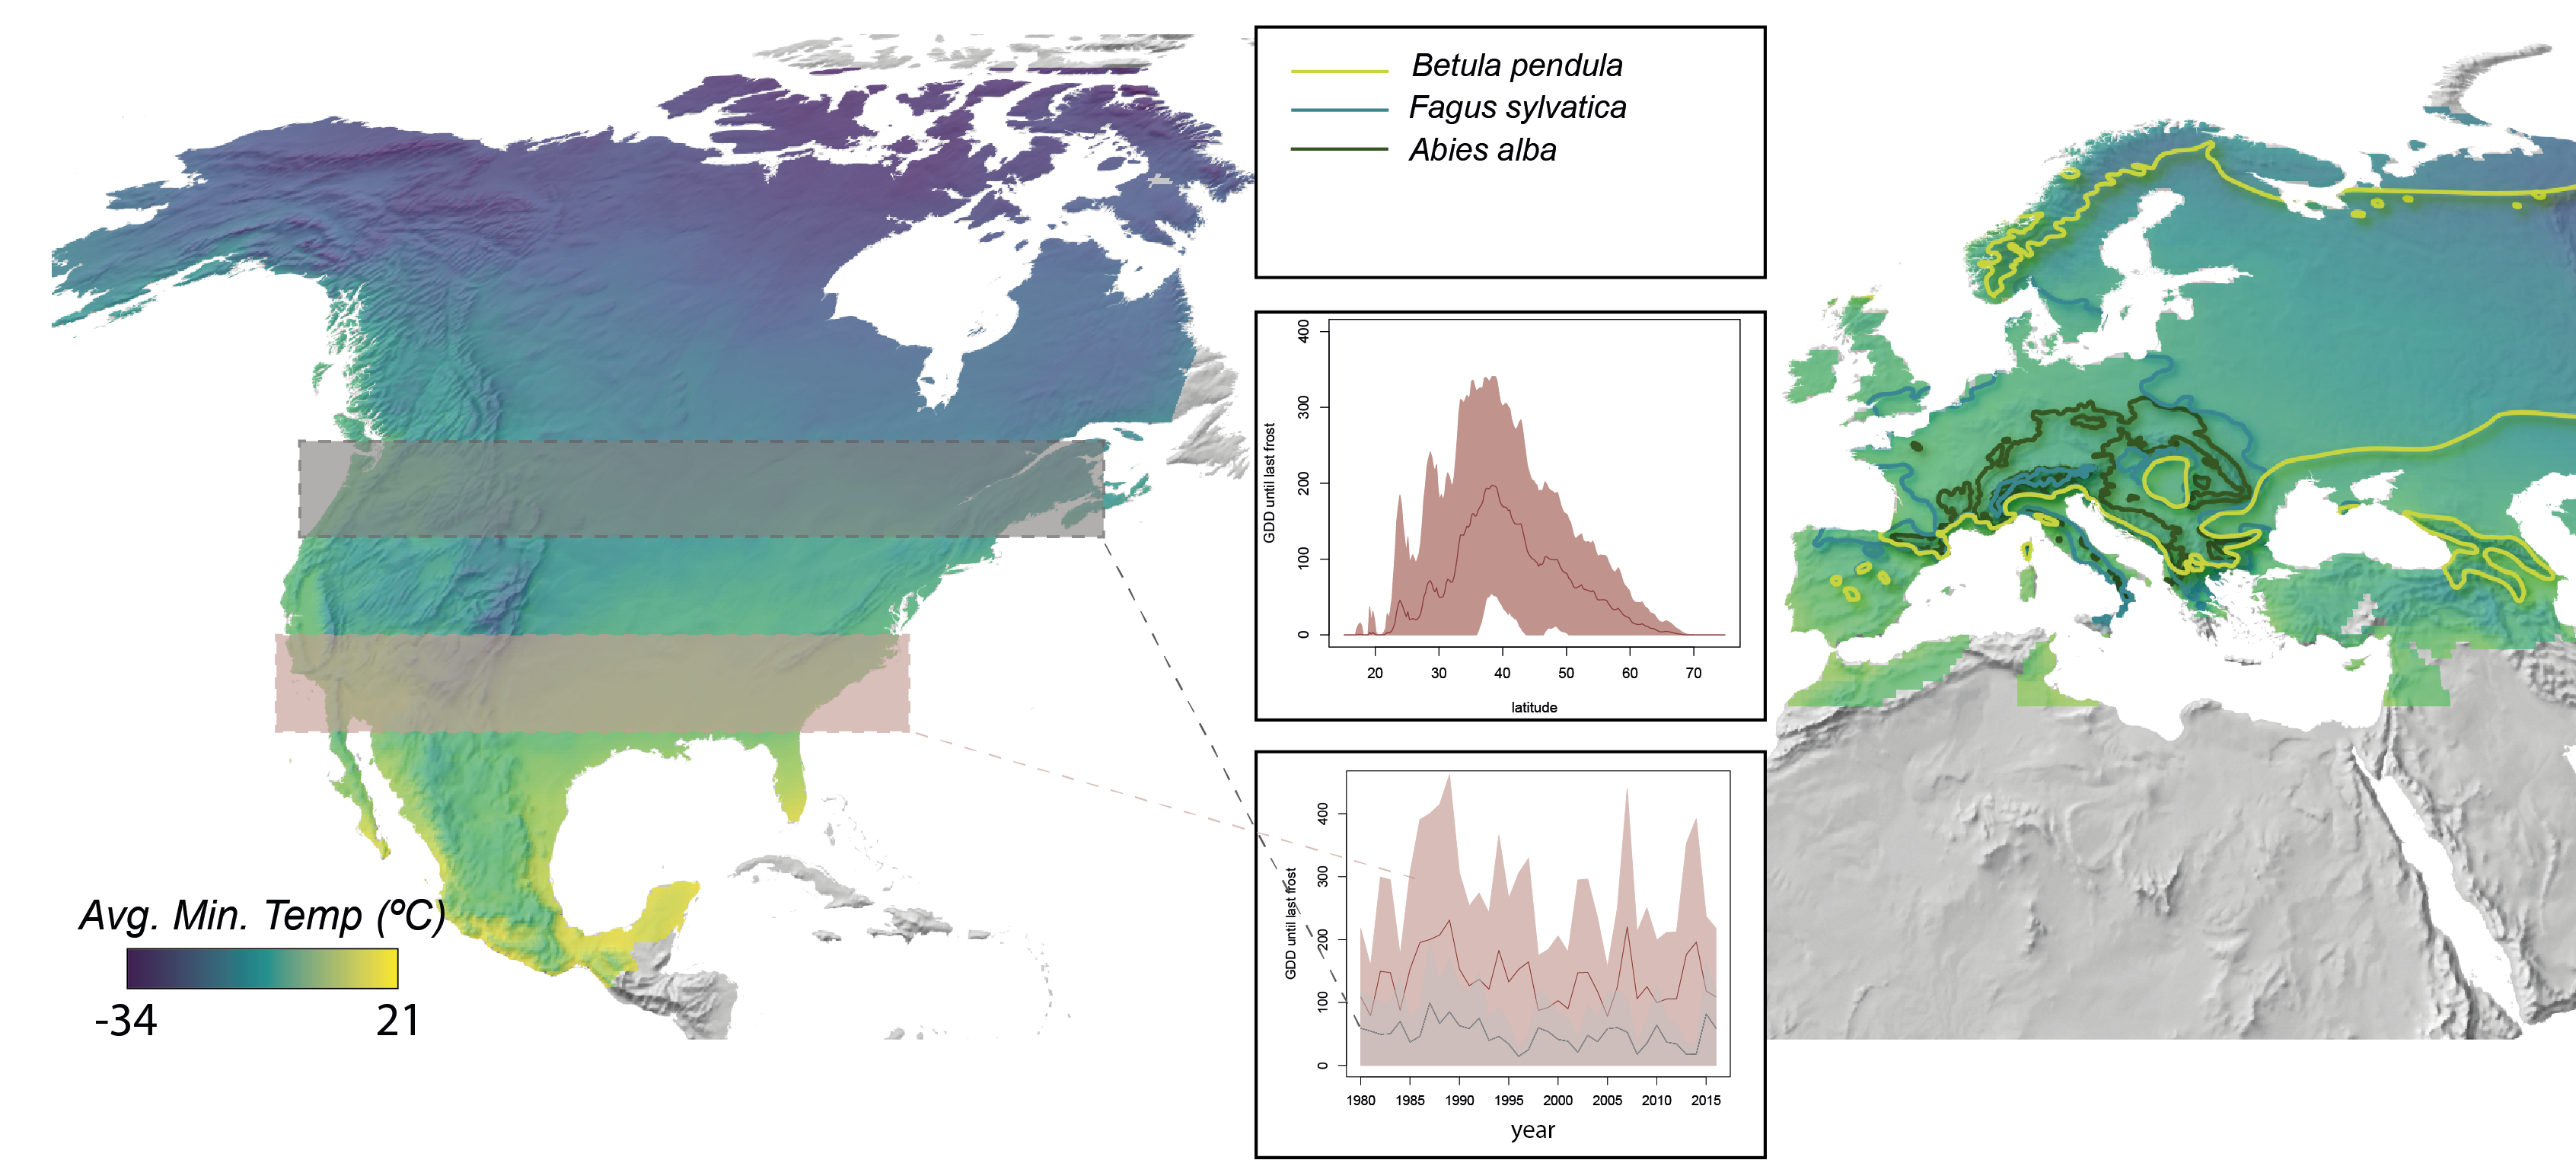
\includegraphics[width=\textwidth]{..//..//analyses/ranges/figures/concept figure draft1.png} 
    \caption{. }
    \label{fig:concept}
\end{figure}

\begin{figure}[h!]
    \centering
 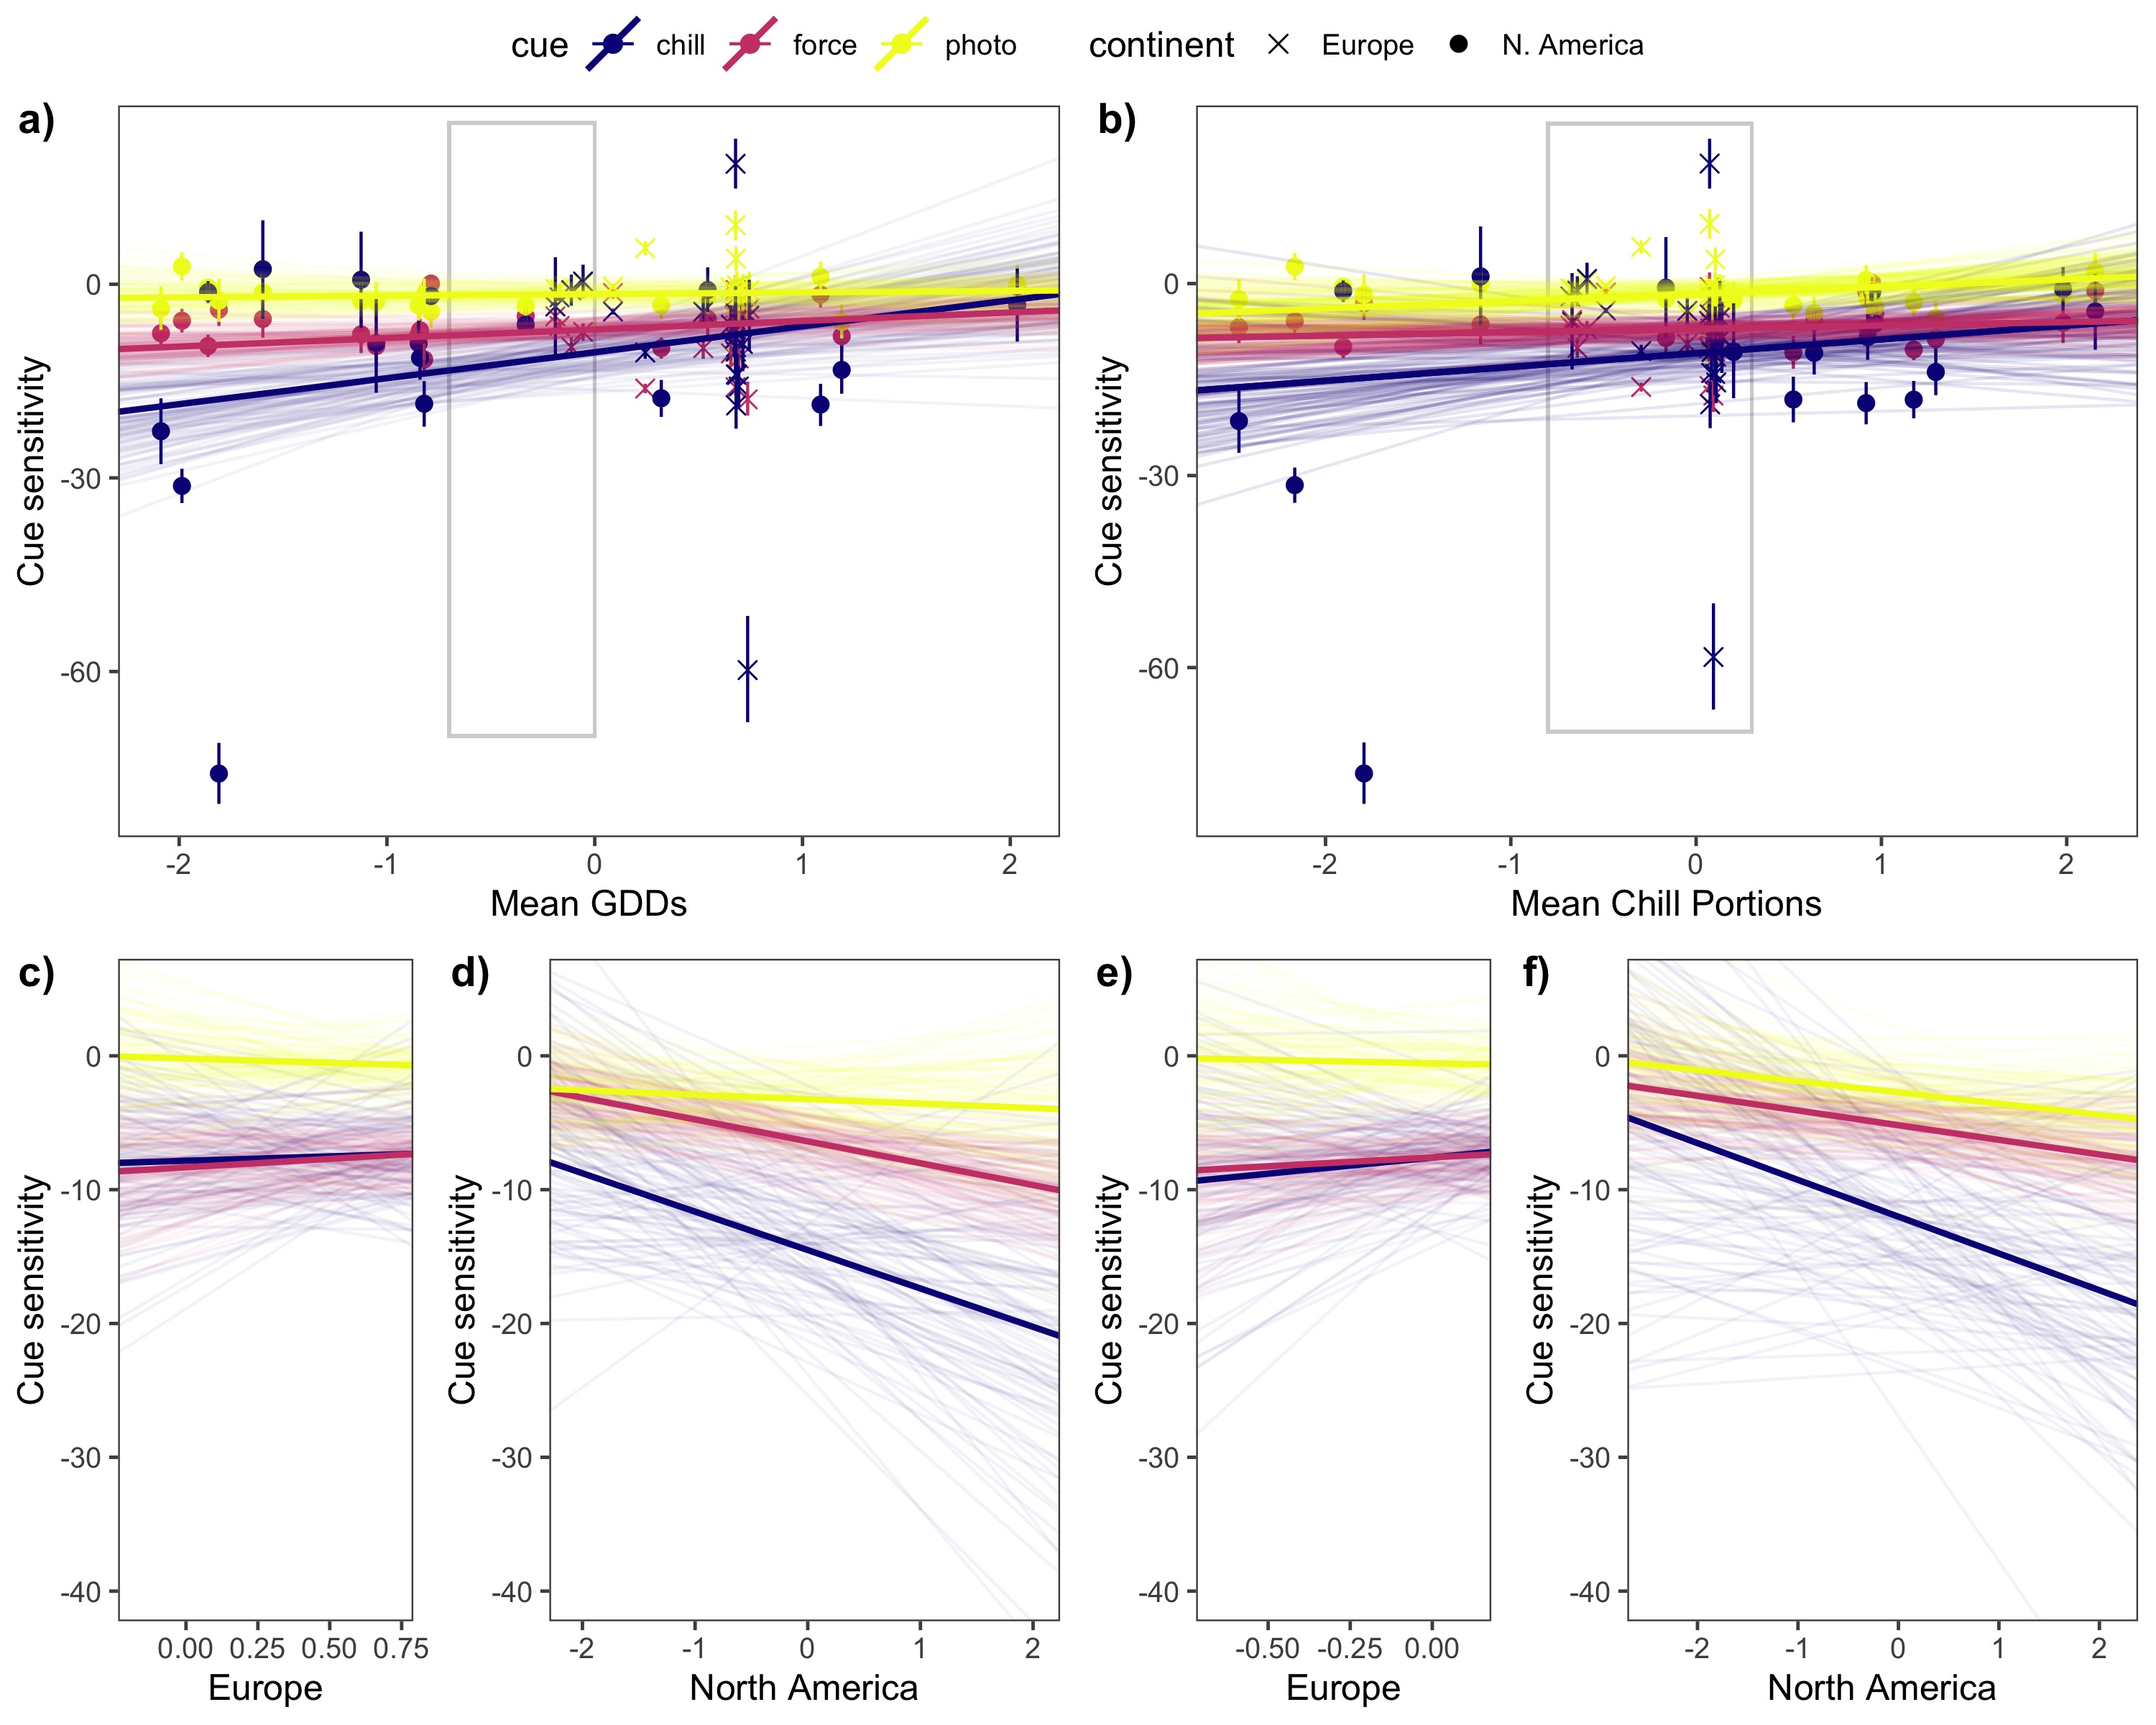
\includegraphics[width=\textwidth]{..//..//analyses/ranges/figures/mock2.jpeg} 
    \caption{The effects of climate intensitives on the phenological sensitivity to chilling, forcing and photoperiod of temperatue woody species. Figure a) depicts the effects of mean GDDs on cue sensitivity for all 40 species in the study and b) depicts effects of chilling on cue sensitivity. All values on the x axis are standardized with zscoring for comparision across plots. The thick, bolded lines indicated the mean estimates of the effect of the climate variables on cue sensitivity estimates and the thinner lines represent 100 random draws from the posterior distrubrion of these estimates to characterize uncertainty. c) and d) depict the relationships between mean GDD and cue sensitivity and e) and f) the relationships between mean chilling and cue sensitivity for models run on only North American species or European species respectivey. }
    \label{fig:mods1}
\end{figure}

\begin{figure}[h!]
    \centering
 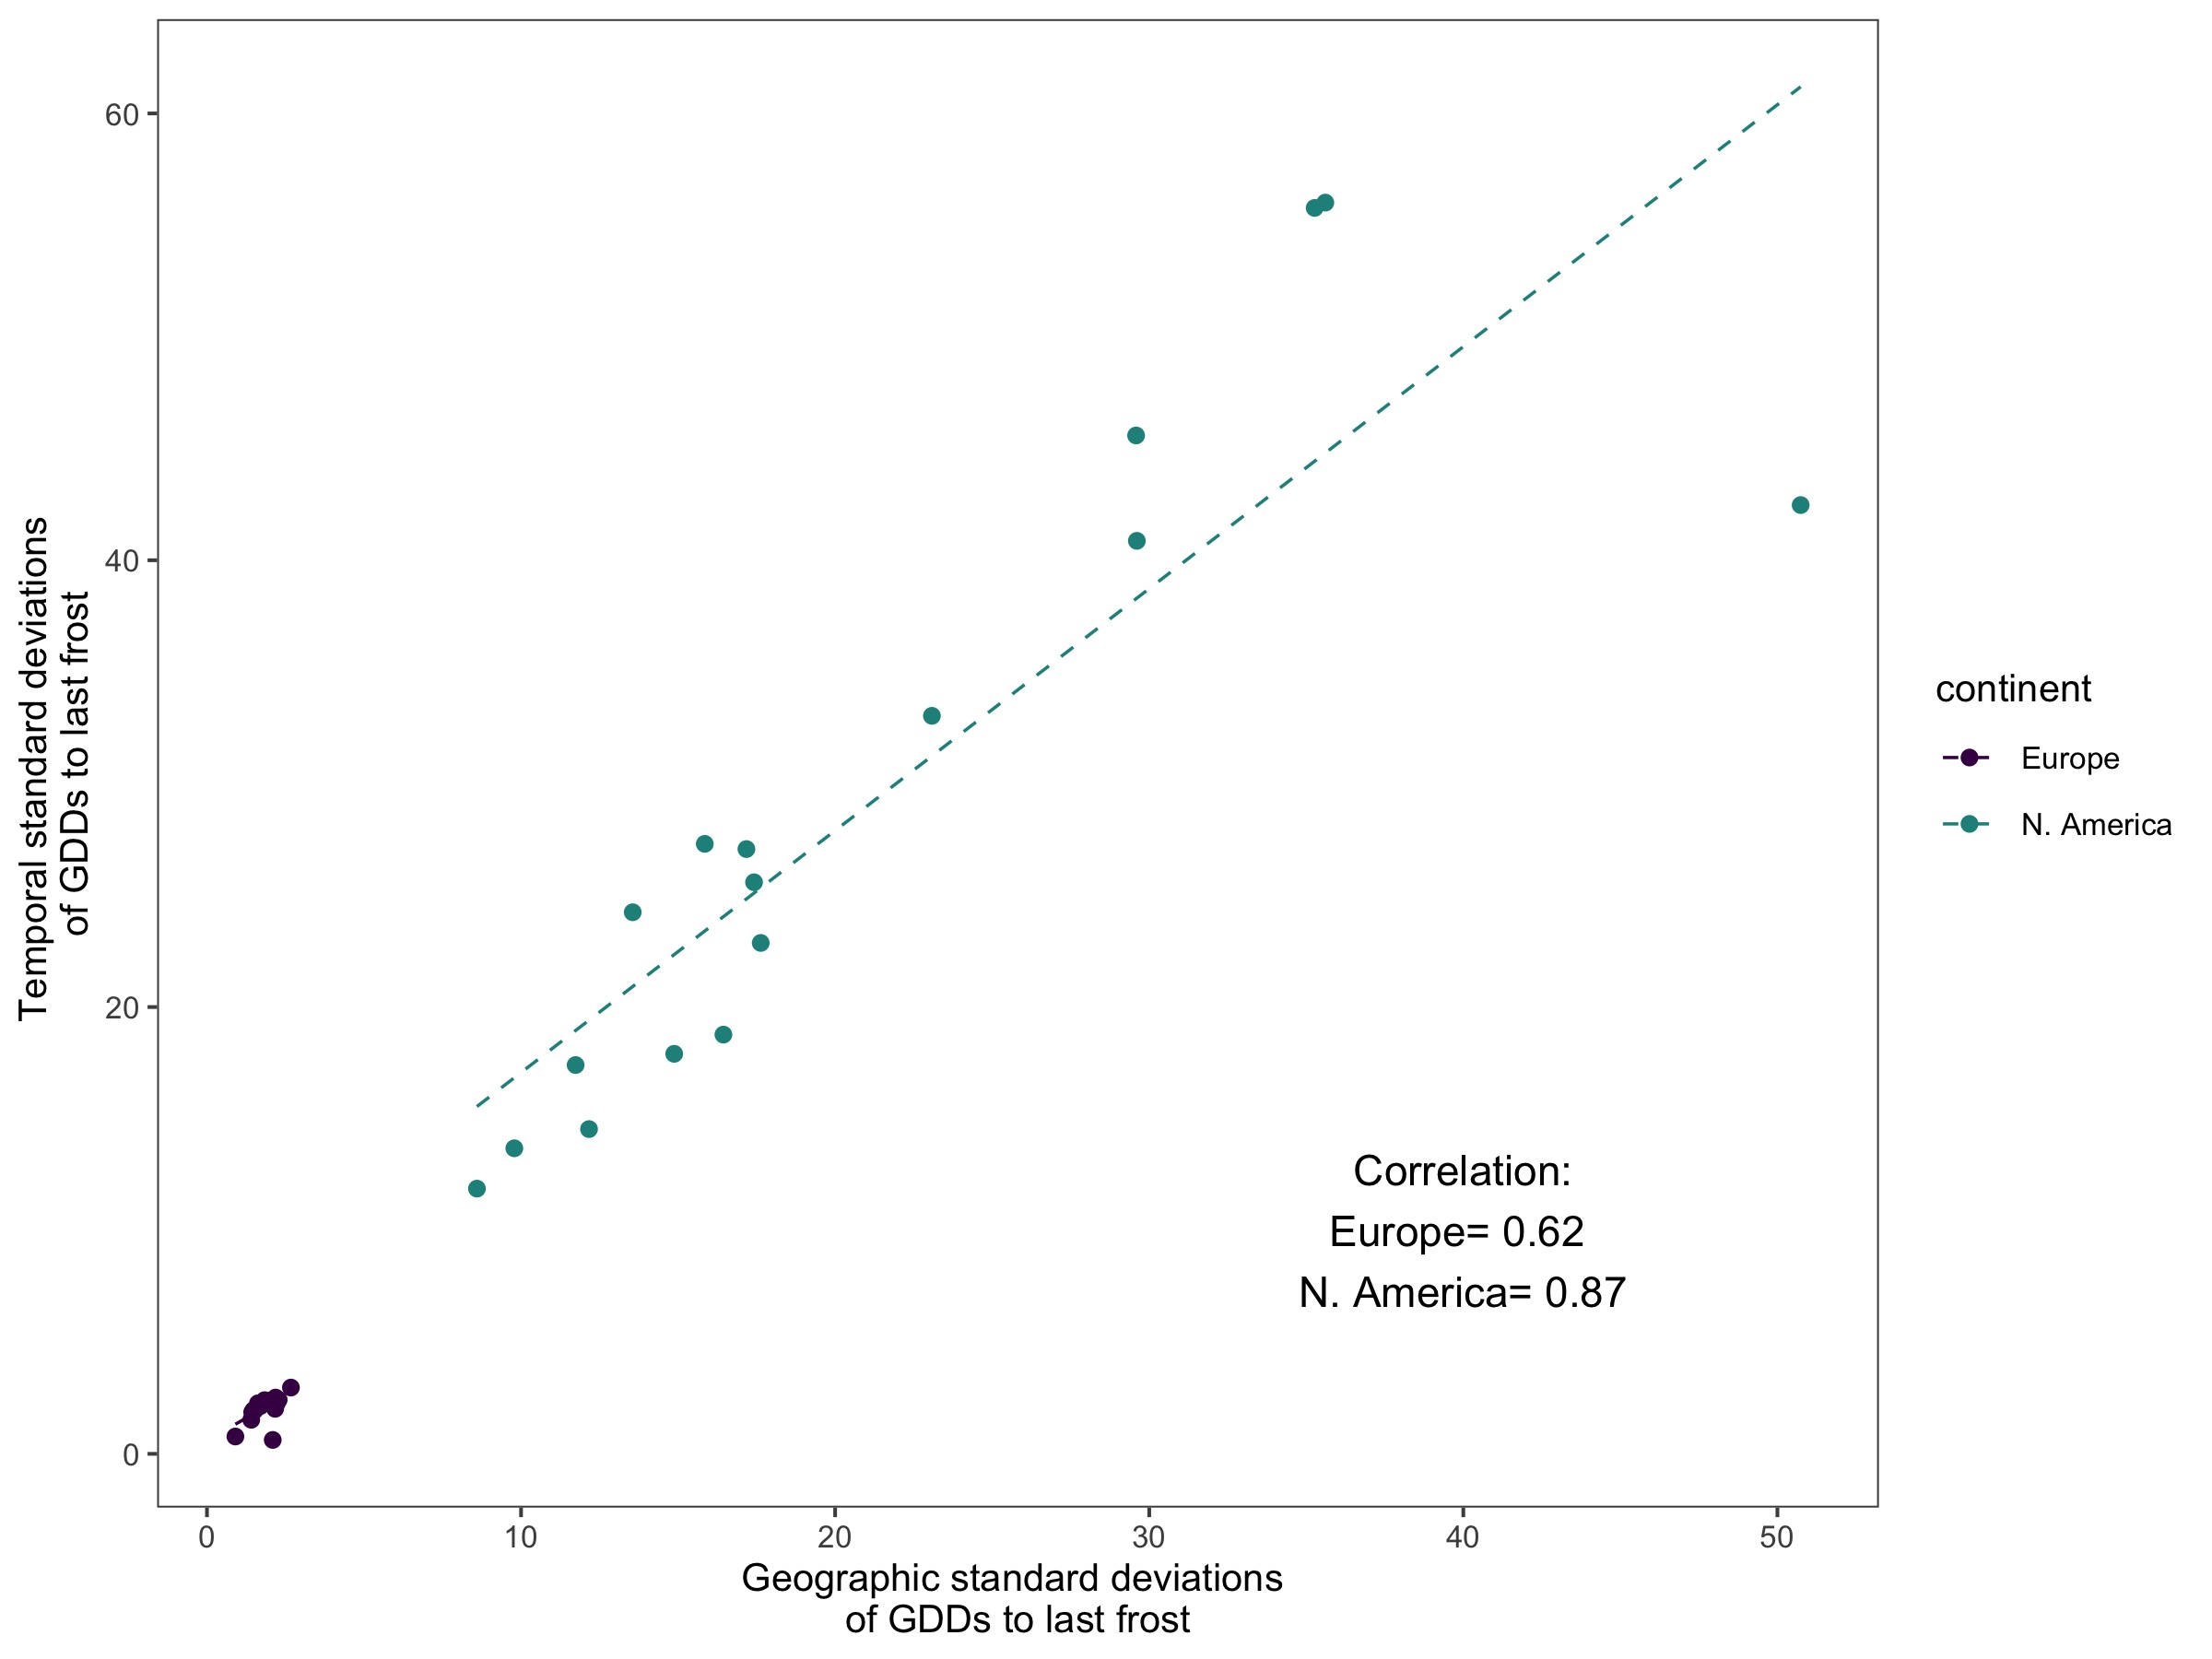
\includegraphics[width=\textwidth]{..//..//analyses/ranges/figures/clim_params.jpeg} 
    \caption{Corelations between spatio-temporal axes of climate varation and intesities in the full data set and across North American and European species ranges. a)  and b) depicts correlation between inter-annual variation in growing degrees to last frost and mean growing degree days and mean levels of chilling in range respectively.  c)  and d) depicts correlation between interannual variation in mean spring temperature (STV) and mean growing degree days and mean levels of chilling in range respectively. e) demonstrate correlations between temporal and spatial inter-annual variation in growing degrees to last frost. f) and g) show the corelations between temporal and spatial variation in GDDs to last frost and STV respectively and h) the correlations between variation in GDDs to last frost and mean number of GDDs to last frost. }
    \label{fig:corrs}
\end{figure}




\begin{figure}[h!]
    \centering
 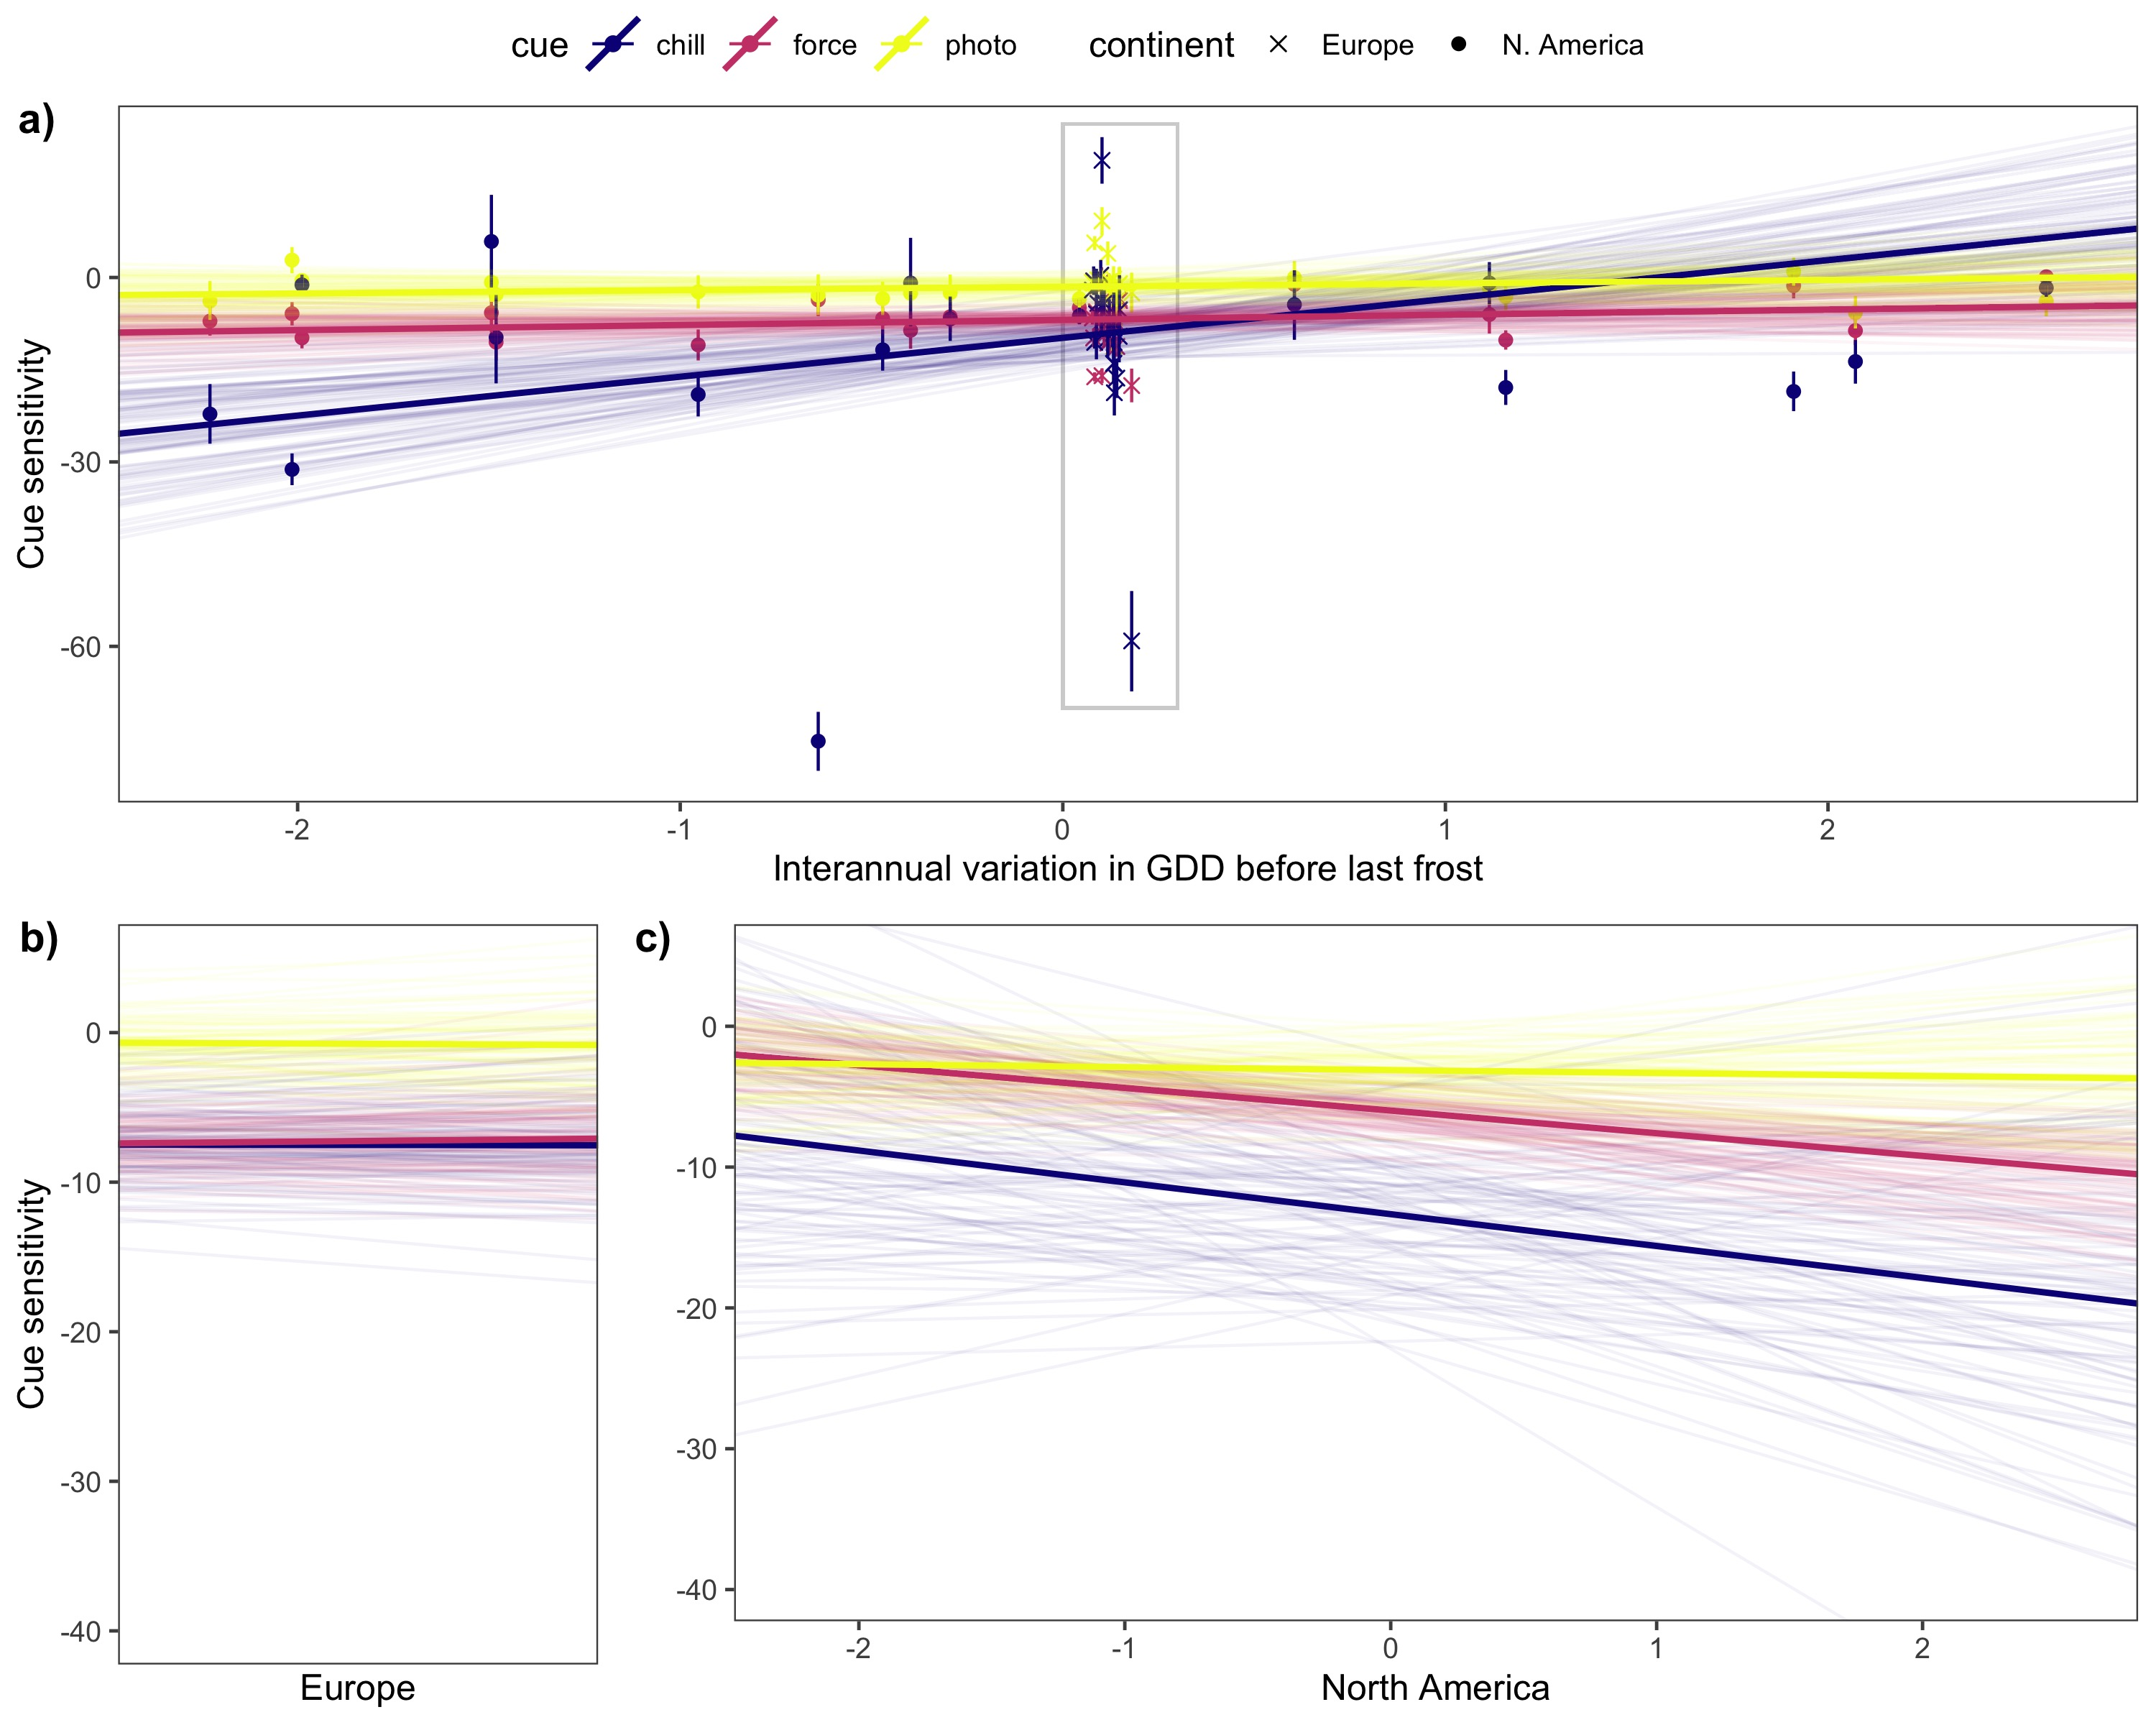
\includegraphics[width=\textwidth]{..//..//analyses/ranges/figures/mock1.jpeg} 
    \caption{ The effects of two measures of spring climate variabilitity on the phenological sensitivity to chilling, forcing and photoperiod of temperatue woody species. Figure a) depicts the effects of variability in number of growing degree days to last frost on cue sensitivity for all 40 species in the study and b) depicts effects of interannual mean spring temperature variation (STV) on cue sensitivity. All values on the x axis are standardized with zscoring for comparision across plots. The thick, bolded lines indicated the mean estimates of the effect of the climate variables on cue sensitivity estimates and the thinner lines represent 100 random draws from the posterior distrubrion of these estimates to characterize uncertainty. c) and d) depict the relationships between variation in GDDs to last frost and cue sensitivity and e) and f) the relationships between STV and cue sensitivity for models run on only North American species or European species respectivey. }
    \label{fig:mods2}
\end{figure}


\begin{figure}[h!]
    \centering
 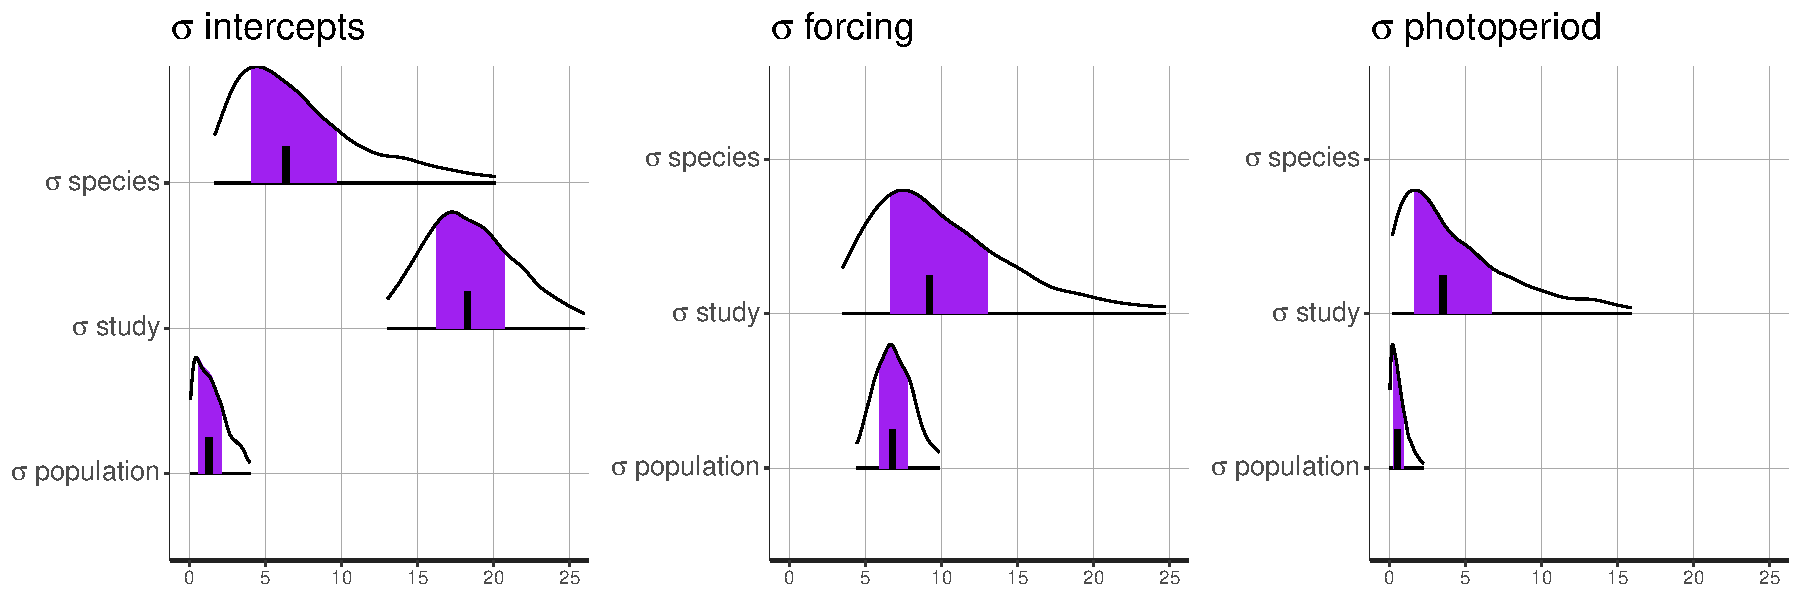
\includegraphics[width=\textwidth]{..//..//analyses/ranges/figures/variancepartitioning.pdf} 
    \caption{Interspecific variation exceeds intraspecific.  Maybe Cat should write this?}
    \label{fig:popy}
\end{figure}

\begin{figure}[h!]
    \centering
 \includegraphics[width=\textwidth]{..//..//analyses/ranges/figures/continental_cues.pdf} 
    \caption{Secondary cues are stronger in North America. Need to check this using new models. }
    \label{fig:cuediff}
\end{figure}

\pagebreak
\iffalse 

\section*{Tables}
\begin{table}
\centering
\begin{tabular}{|r|rrr|rrr|rrr|}
  \hline
  climate & Forcing & 10\% & 90\% & Photo & 10\% & 90\% & Chill & 10\% & 90\% \\ 
  \hline
 Mean Chill Portions & 1.43 & -1.70 & 4.53 & 0.53 & -2.61 & 3.74 & 3.10 & -0.17 & 6.44 \\ 
  Mean GDDs & 0.11 & -0.96 & 1.24 & 1.32 & 0.16 & 2.47 & 3.28 & 0.27 & 6.25 \\ 
   STV & -0.68 & -1.90 & 0.55 & 0.66 & -0.51 & 1.84 & 3.41 & 0.18 & 6.74 \\ 
   Var. GGD to last frost & -1.18 & -2.58 & 0.22 & 1.41 & 0.01 & 2.81 & 2.40 & -1.24 & 5.99 \\ 
   \hline
\end{tabular}
\label{tab:outfull}
\caption{}
\end{table}

\begin{table}
\centering
\begin{tabular}{|r|p{3 cm}|rrr|rrr|rrr|}
  \hline
  \hline
 continent & climate & Forcing & 10\% & 90\% & Photo & 10\% & 90\% & Chill & 10\% & 90\% \\ 
  \hline
 Eu & Mean Chill Portions & 1.84 & -1.45 & 5.09 & 0.20 & -3.03 & 3.43 & 1.85 & -1.53 & 5.24 \\ 
 \hline
    Eu & Mean GDDs & 3.24 & -5.47 & 11.63 & -0.50 & -9.13 & 8.19 & 4.05 & -6.78 & 14.92 \\ 
    \hline
    Eu & STV & 1.47 & -11.11 & 14.13 & -2.22 & -14.61 & 10.58 & 0.92 & -11.64 & 13.61 \\ 
    \hline
    Eu & Var. GGD to last frost & 3.67 & -7.73 & 14.81 & 0.11 & -10.95 & 10.87 & 3.30 & -7.94 & 14.36 \\ 
    \hline
    \hline
    N.A & Mean Chill Portions & 0.69 & -2.55 & 3.92 & 0.46 & -2.78 & 3.58 & 3.90 & 0.24 & 7.53 \\ 
    \hline
    N.A & Mean GDDs & -1.48 & -2.43 & -0.52 & -0.31 & -1.58 & 0.88 & -3.65 & -6.92 & -0.31 \\ 
    \hline
    N.A & STV & -1.29 & -2.57 & -0.05 & -0.38 & -1.99 & 1.18 & 1.12 & -2.71 & 4.94 \\ 
    \hline
    N.A & Var. GGD to last frost & -3.07 & -4.97 & -1.09 & -0.46 & -2.90 & 1.99 & -5.94 & -11.55 & -0.24 \\ 
  \hline
   \hline
\end{tabular}
\label{tab:outcont}
\caption{}
\end{table}

\begin{table}[ht]
\centering
\begin{tabular}{rrrrrrl}
  \hline
 & mean & 10\% & 25\% & 75\% & 90\% & continent \\ 
  \hline
muChillSp & -5.66 & -12.59 & -9.28 & -2.05 & 1.28 & Eu \\ 
  muPhotoSp & -0.52 & -7.10 & -3.88 & 2.95 & 5.84 & Eu \\ 
  muForceSp & -5.48 & -12.42 & -8.86 & -1.99 & 1.36 & Eu \\ 
  muChillSp1 & -7.91 & -15.30 & -11.74 & -4.05 & -0.59 & N.A \\ 
  muPhotoSp1 & -2.59 & -5.75 & -4.21 & -0.96 & 0.57 & N.A \\ 
  muForceSp1 & -2.43 & -4.91 & -3.65 & -1.16 & -0.04 & N.A \\ 
   \hline
\end{tabular}
\caption{}
\end{table}
\fi 

\end{document}
